\subsection{Completed Result Overview}

Figure~\ref{fig:gld-result-overview} replaces the oversized full-results table with a compact visual summary of the completed GLD comparisons.
Panel A shows the shared locked-setting baselines, Panel B shows the source-optimized imported baselines, and Panel C shows the best completed Mamba-HPO variants.
All curves are plotted on the original GLD price scale using RMSE. The complete machine-readable records remain available in the result CSV files under \texttt{results/}.

\begin{figure}[t]
\centering
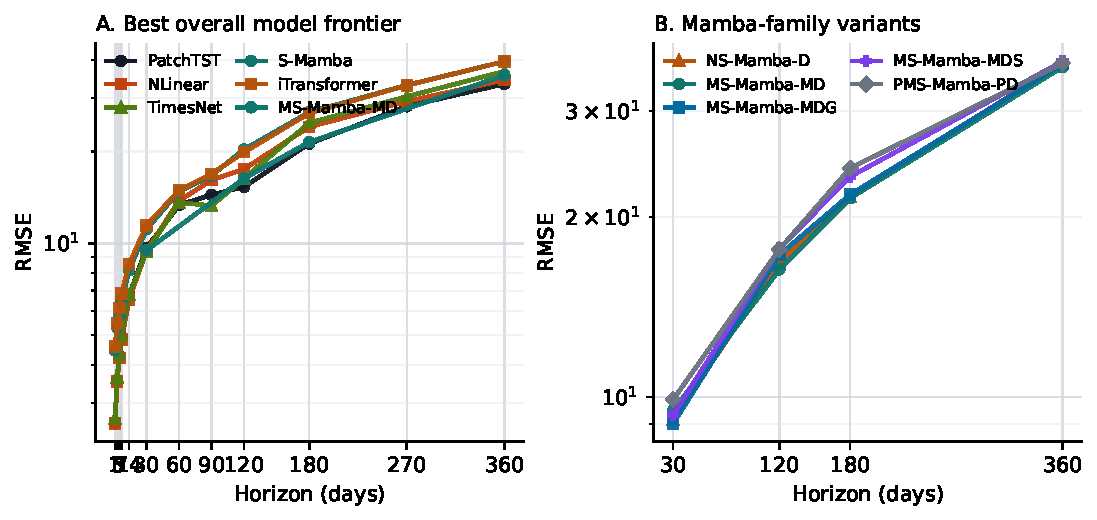
\includegraphics[width=\linewidth]{figures/gld_result_overview.pdf}
\caption{Completed GLD RMSE comparison across the three main evaluation tracks. Panel A: shared locked-setting baselines over all 12 horizons. Panel B: source-optimized imported baselines over all 12 horizons. Panel C: best completed Mamba-HPO variants over the currently completed diagnostic horizons 30, 120, 180, and 360 days. The figure makes the main ranking structure visible without the space cost of a full longtable.}
\label{fig:gld-result-overview}
\end{figure}

